%!TEX program = xelatex
\documentclass[11pt]{beamer}

\usepackage{amsfonts}
\usepackage{amsmath}
\usepackage{blindtext}
\usepackage{enumitem}

\usetheme{SaoPaulo}

\title{Python Basics!}
\subtitle{arguments, parameters, methods, comments}
\author{CS101 Lecture \#5}
\date{2016-09-07}

\setcounter{showSlideNumbers}{1}

\begin{document}
  \setcounter{showProgressBar}{0}
  \setcounter{showSlideNumbers}{0}

%%%%%%%%%%%%%%%%%%%%%%%%%%%%%%%%%%%%%%%%%%%%%%%%%%%%%%%%%%%%%%%%%%%%%%%%%%%%%%%%
\frame{\titlepage}

%%%%%%%%%%%%%%%%%%%%%%%%%%%%%%%%%%%%%%%%%%%%%%%%%%%%%%%%%%%%%%%%%%%%%%%%%%%%%%%%
\setcounter{framenumber}{0}
\setcounter{showProgressBar}{1}
\setcounter{showSlideNumbers}{1}

%%%%%%%%%%%%%%%%%%%%%%%%%%%%%%%%%%%%%%%%%%%%%%%%%%%%%%%%%%%%%%%%%%%%%%%%%%%%%%%%
\section{Administrivia}

%%%%%%%%%%%%%%%%%%%%%%%%%%%%%%%%%%%%%%%%%%%%%%%%%%%%%%%%%%%%%%%%%%%%%%%%%%%%%%%%
\begin{frame}
  \frametitle{Administrivia}
  \Enlarge
  \begin{itemize}
  \myitem  Homework \#2 is due Friday Sep.\ 9.
  \myitem  Labs resume next week.
  \end{itemize}
\end{frame}

%%%%%%%%%%%%%%%%%%%%%%%%%%%%%%%%%%%%%%%%%%%%%%%%%%%%%%%%%%%%%%%%%%%%%%%%%%%%%%%%
\section{Warmup Quiz}

%%%%%%%%%%%%%%%%%%%%%%%%%%%%%%%%%%%%%%%%%%%%%%%%%%%%%%%%%%%%%%%%%%%%%%%%%%%%%%%%
\begin{frame}[fragile]
  \frametitle{Question \#1}
  \Enlarge

  \begin{semiverbatim}
s = '%s' + 'i'
i = 3 / 6
x = float(s%i) * 2
  \end{semiverbatim}
  What is the value of \texttt{x}?
  \begin{enumerate}[label=\Alph*]
  \item  \texttt{0.0}
  \item  \texttt{'\%i\%i'}
  \item  \texttt{1.0}
  \item  \texttt{'1.0'}
  \end{enumerate}
\end{frame}

%%%%%%%%%%%%%%%%%%%%%%%%%%%%%%%%%%%%%%%%%%%%%%%%%%%%%%%%%%%%%%%%%%%%%%%%%%%%%%%%
\begin{frame}[fragile]
  \frametitle{Question \#2}
  \Enlarge

  \begin{semiverbatim}
s = "WATER MAIN"[2:6]
t = int(3.7)
x = s[-1] + s[t-2]
  \end{semiverbatim}
  What is the value of \texttt{x}?
  \begin{enumerate}[label=\Alph*]
  \item  \texttt{"NA"}
  \item  \texttt{" E"}
  \item  \texttt{" R"}
  \item  \texttt{"ME"}
  \end{enumerate}
\end{frame}

%%%%%%%%%%%%%%%%%%%%%%%%%%%%%%%%%%%%%%%%%%%%%%%%%%%%%%%%%%%%%%%%%%%%%%%%%%%%%%%%
\begin{frame}[fragile]
  \frametitle{Question \#3 (Worked)}
  \Enlarge

  \begin{semiverbatim}
s = "WATER MAIN"[2:6]
    #0123456789
s =   "TER "
t = int(3.7)
t = 3
x = s[-1] + s[t-2]
x = " "   + "E"
x = " E"
  \end{semiverbatim}
\end{frame}

%%%%%%%%%%%%%%%%%%%%%%%%%%%%%%%%%%%%%%%%%%%%%%%%%%%%%%%%%%%%%%%%%%%%%%%%%%%%%%%%
\begin{frame}[fragile]
  \frametitle{Question \#4}
  \Enlarge

  \begin{semiverbatim}
i = len("WATER MAIN")
c = (1.0 + 2.0j) * (-i)
x = abs( min( c.real,-13 ) )
  \end{semiverbatim}
  What is the value of \texttt{x}?
  \begin{enumerate}[label=\Alph*]
  \item  \texttt{0}
  \item  \texttt{11}
  \item  \texttt{12}
  \item  \texttt{13}
  \end{enumerate}
\end{frame}

%%%%%%%%%%%%%%%%%%%%%%%%%%%%%%%%%%%%%%%%%%%%%%%%%%%%%%%%%%%%%%%%%%%%%%%%%%%%%%%%
\section{Functions Redux}

%%%%%%%%%%%%%%%%%%%%%%%%%%%%%%%%%%%%%%%%%%%%%%%%%%%%%%%%%%%%%%%%%%%%%%%%%%%%%%%%
\begin{frame}
  \frametitle{Functions}
  \Enlarge

  \begin{itemize}
  \myitem  A small program (block of code) we can run within Python.
    \begin{itemize}
    \mysubitem  Saves us from rewriting code
    \mysubitem  Don't reinvent the wheel!
    \end{itemize}
  \myitem  Analogy:  Functions are more verbs.
  \myitem  Also called subroutine or procedure.
  \end{itemize}
\end{frame}

%%%%%%%%%%%%%%%%%%%%%%%%%%%%%%%%%%%%%%%%%%%%%%%%%%%%%%%%%%%%%%%%%%%%%%%%%%%%%%%%
\begin{frame}
  \frametitle{Function calls}
  \Enlarge

  \begin{itemize}
  \myitem  When we want to execute a function, we call or invoke it.
  \myitem  Use name of the function with parentheses.
    \begin{itemize}
    \mysubitem  \texttt{print()}
    \end{itemize}
  \myitem  Many functions come built-in to Python or in the standard library.
  \myitem  Others we will compose at need.
  \end{itemize}
\end{frame}

%%%%%%%%%%%%%%%%%%%%%%%%%%%%%%%%%%%%%%%%%%%%%%%%%%%%%%%%%%%%%%%%%%%%%%%%%%%%%%%%
\begin{frame}
  \frametitle{User input}
  \Enlarge

  \begin{itemize}
  \myitem  \texttt{input} is a built-in function.
  \myitem  Argument:  string prompting user
  \myitem  Return value:  input from user (as \texttt{str})
  \end{itemize}
\end{frame}

%%%%%%%%%%%%%%%%%%%%%%%%%%%%%%%%%%%%%%%%%%%%%%%%%%%%%%%%%%%%%%%%%%%%%%%%%%%%%%%%
\begin{frame}
  \frametitle{Goal}
  \Enlarge

  \begin{itemize}
  \myitem  A program should achieve a goal. %\pause
  \myitem  Let's implement the quadratic equation.
  \end{itemize}
\end{frame}

%%%%%%%%%%%%%%%%%%%%%%%%%%%%%%%%%%%%%%%%%%%%%%%%%%%%%%%%%%%%%%%%%%%%%%%%%%%%%%%%
\begin{frame}[fragile]
  \frametitle{Example:  Quadratic equation}

  \begin{semiverbatim}
print( "QUADRATIC SOLVER" )
print( "a x^2 + b x + c = 0" )

a = float( input( 'a: ' ) )
b = float( input( 'b: ' ) )
c = float( input( 'c: ' ) )

root = ( b**2 - 4*a*c ) ** 0.5
denom = 2 * a

pos = (-b + root) / denom
neg = (-b - root) / denom

message1 = "%.2f + %.2fi" % (pos.real,pos.imag)
message2 = "%.2f + %.2fi" % (neg.real,neg.imag)

print("Solution 1: %s" % message1)
print("Solution 2: %s" % message2)
  \end{semiverbatim}
\end{frame}

%%%%%%%%%%%%%%%%%%%%%%%%%%%%%%%%%%%%%%%%%%%%%%%%%%%%%%%%%%%%%%%%%%%%%%%%%%%%%%%%
\begin{frame}
  \frametitle{Achievement unlocked!}
  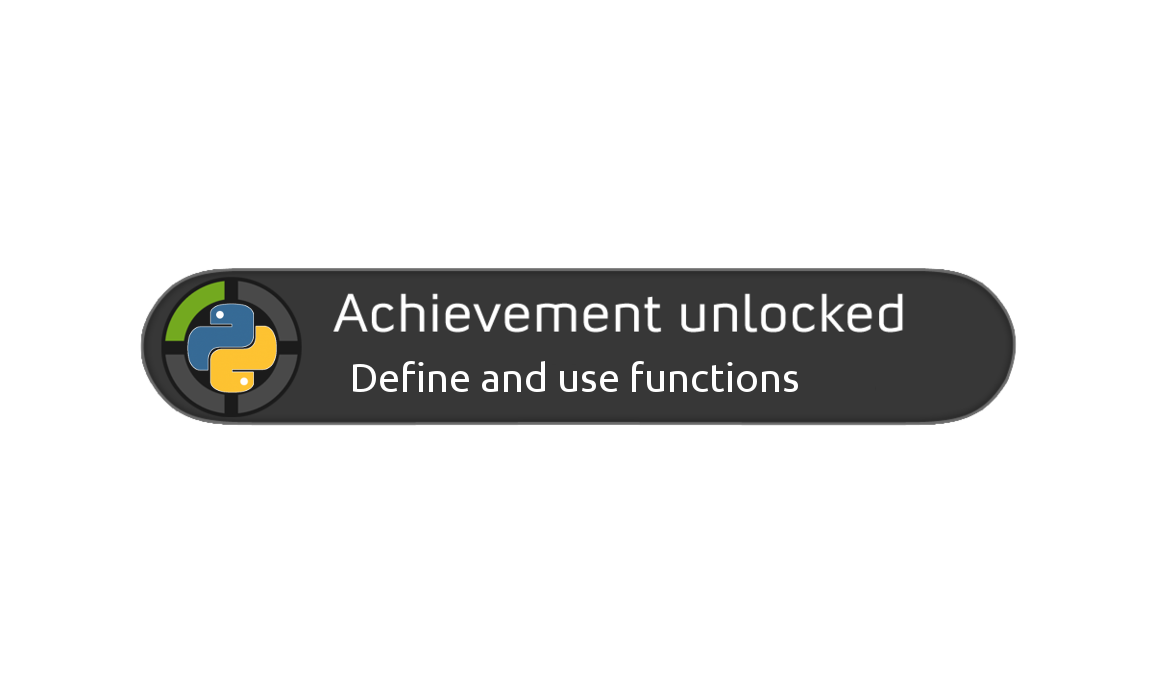
\includegraphics[width=\textwidth]{./img/achievement_unlocked-functions.png}
\end{frame}

%%%%%%%%%%%%%%%%%%%%%%%%%%%%%%%%%%%%%%%%%%%%%%%%%%%%%%%%%%%%%%%%%%%%%%%%%%%%%%%%
\section{Methods}

%%%%%%%%%%%%%%%%%%%%%%%%%%%%%%%%%%%%%%%%%%%%%%%%%%%%%%%%%%%%%%%%%%%%%%%%%%%%%%%%
\begin{frame}[fragile]
  \frametitle{Methods}
  \Enlarge

  \begin{itemize}
  \myitem  Like attributes, functions can be stored inside a type as well. %\pause
  \myitem  Use attribute operator on the value. %\pause
    \begin{semiverbatim}
"STOP SHOUTING!".lower()
(1 + 1j).conjugate()
    \end{semiverbatim} %\pause
  \myitem  Value is treated like an argument.
  \end{itemize}
\end{frame}

%%%%%%%%%%%%%%%%%%%%%%%%%%%%%%%%%%%%%%%%%%%%%%%%%%%%%%%%%%%%%%%%%%%%%%%%%%%%%%%%
\begin{frame}[fragile]
  \frametitle{String methods}
  \Enlarge

  \begin{semiverbatim}
"GATTACA".count('A')
"MVEMJSUN".find('J')
"ABACADABRA".replace('AB','G')
' FNORD '.strip()
'high king of narnia'.title()
'wEiRd'.swapcase()
  \end{semiverbatim}
\end{frame}

%%%%%%%%%%%%%%%%%%%%%%%%%%%%%%%%%%%%%%%%%%%%%%%%%%%%%%%%%%%%%%%%%%%%%%%%%%%%%%%%
\begin{frame}[fragile]
  \frametitle{Example}
  \Enlarge

  \begin{semiverbatim}
s = "WATER MAIN"
x = s[ 0:s.find( ' ' ) ].lower()
x = x.title().swapcase()
  \end{semiverbatim}
  What is the value of \texttt{x}?
  \begin{enumerate}[label=\Alph*]
  \item  \texttt{'wATER'}
  \item  \texttt{'Water'}
  \item  \texttt{'wATE'}
  \item  \texttt{'aTER'}
  \end{enumerate}
\end{frame}

%%%%%%%%%%%%%%%%%%%%%%%%%%%%%%%%%%%%%%%%%%%%%%%%%%%%%%%%%%%%%%%%%%%%%%%%%%%%%%%%
\section{Comments}

%%%%%%%%%%%%%%%%%%%%%%%%%%%%%%%%%%%%%%%%%%%%%%%%%%%%%%%%%%%%%%%%%%%%%%%%%%%%%%%%
\begin{frame}[fragile]
  \frametitle{Methods}
  \Enlarge

  \begin{itemize}
  \myitem  We can explain our code using comments. %\pause
  \myitem  Comments begin with a \texttt{\#} sign; Python ignore the rest of the line. %\pause
  \myitem  Long comments can also be stored as triple-quoted strings. %\pause
    \begin{semiverbatim}
dx = 0.01  # grid spacing, m
V  = 14.2  # voltage, V
"""
This is an extended comment.
I can be many lines long.
Use me to explain functions or formulae, to document code,
or to temporarily hide blocks you don't want to run.
"""
    \end{semiverbatim}
  \end{itemize}
\end{frame}

%%%%%%%%%%%%%%%%%%%%%%%%%%%%%%%%%%%%%%%%%%%%%%%%%%%%%%%%%%%%%%%%%%%%%%%%%%%%%%%%
\section{Reminders}

%%%%%%%%%%%%%%%%%%%%%%%%%%%%%%%%%%%%%%%%%%%%%%%%%%%%%%%%%%%%%%%%%%%%%%%%%%%%%%%%
\begin{frame}
  \frametitle{Reminders}
  \Enlarge

  \begin{itemize}
  \myitem  Homework \#2 is due Friday Sep.\ 9.
  \myitem  Labs resume next week.
  \end{itemize}
\end{frame}

\end{document}
